\chapter{AI-Greyboxing}
\label{cha:GreyBoxing}
Der erste Ansatz der verfolgt wurde, wird im folgenden \textit{GreyBoxing} genannt.
\section{Konzept}
\label{sec:KonzeptGreyBoxing}
Das Konzept ist hierbei, dass über einen Generator zufällige Nicht-Straßenbilder erzeugt werden, diese von der Schnittstelle bewertet werden, und eine zweite, lokale AI auf die Scores der Schnittstelle trainiert werden. 
~\newline
Mit fortschreitendem Experiment sollte die lokale AI ihr Verhalten an das der Schnittstelle angleichen und als Greybox dienen: Die lokal erzeugten Bilder und die lokalen Scores, wären ähnlich zu den Scores der Schnittstelle. 

Ist dieser Zustand erreicht, kann man lokal Bilder generieren, und sobald die GreyBox dieses akkzeptiert an die Schnittstelle schicken. 

Die doppelt-bewerteten Ergebnisse können erneut ins Training einfließen, um die GreyBox weiter zu verbessern. 

~\newline Ausgehend hiervon kann ebenfalls weitere Verbesserung am Generator vorgenommen werden, und lokal getestet werden.
Man kann somit den Generator ebenfalls \textit{trainieren} und gegebenenfalls Hyperparamter wie Farbanteile oder Helligkeit anpassen. 

~\newline Das Konzept umfasst im erweiterten Sinn ebenfalls alle Maßnahmen, um die stetige, iterative Verbesserung der beteiligten Komponenten zu vollziehen.      

~\newline Als Generator wurde für die Implementierung einfaches Rauschen gewählt. Andere mögliche Generatoren sind z.B. Webcrawler, welche Bilder nach gewissen Parametern aussuchen, oder Generatoren welche ein Bild lediglich \textit{verzerren}, wie das in der Degeneration in Kapitel \ref{cha:Degeneration} der Fall ist. 

\section{Implementierung und erste Ergebnisse}
\label{sec:ImplementierungGreyBoxing}
\begin{figure}[h]
	\centering
	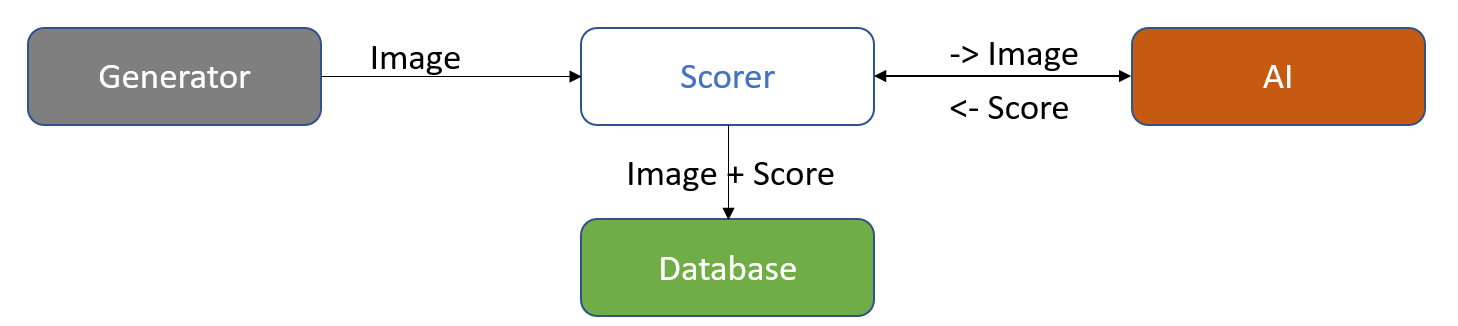
\includegraphics[width=0.9\linewidth]{Images/GreyBoxingStart}
	\caption[Komponenten Setup-Phase]{Komponenten Setup-Phase}
	\label{fig:greyboxingstart}
\end{figure}

Die Abbildung \ref{fig:greyboxingstart} zeigt den ersten Überblick über die \textit{Setup-Phase} des Greyboxing:

\paragraph{Generator:} produziert zufällige Bilder auf Abruf. Innerhalb des ersten Ansatzes wurde der Generator als einfaches Pythonfile mit wenigen Methoden umgesetzt.  
\paragraph{Scorer:} erhält Bilder vom Generator, lässt sie von der Schnittstelle bewerten, und speichert die Ergebnisse samt Bild in einer Datenbank. 

Die Hauptlogik findet somit im Scorer statt. Er wurde als Jupyternotebook umgesetzt.
\paragraph{AI:} Die Trasi-Schnittstelle, wie in Abschnitt \ref{sec:EigenschaftenTrasi} beschrieben.
\paragraph{Database:} eine Datenbank, die Bilder und Scores abspeichert.
In der Implementierung wurde eine MongoDB gewählt, welche sich gut eignete um die JSON-Antworten der Schnittstelle direkt zu verwalten. 
~\newline
Mit dieser Architektur wurden über einen längeren Zeitraum knapp 100 000 Bilder gesammelt und abgespeichert. 
~\newline
Nachdem die Daten gesammelt wurden, sollte eine AI trainiert werden, welche die Scores der Schnittstelle imitiert. 

Hierfür wurde Tensorflow gewählt, und verschiedene Modell-konfigurationen sowie Hyperparameter durchgespielt. 
Es konnte kein zufriedenstellendes Modell erzeugt werden, weiterführend hierzu in Abschnitt \ref{sec:ProblemGreyBoxing}.

~\newline Unabhängig davon soll noch einmal das Konzept nach dem Training vorgestellt werden, dargestellt in Abbildung \ref{fig:greyboxingrunning}: 
 \begin{figure}[h]
 	\centering
 	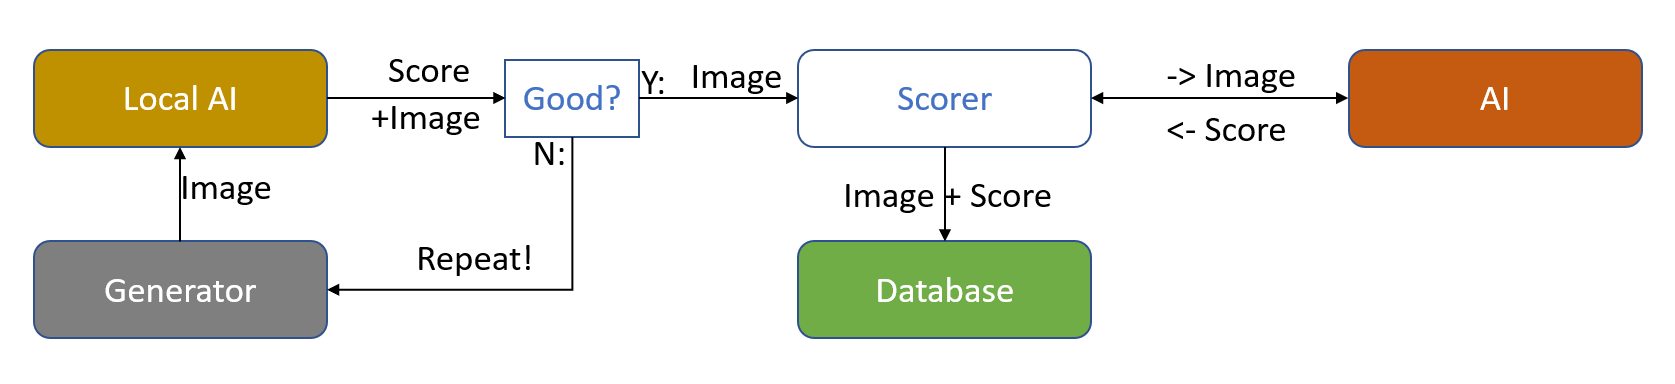
\includegraphics[width=0.9\linewidth]{Images/GreyBoxingRunning}
 	\caption{Komponenten Betriebs-Phase}
 	\label{fig:greyboxingrunning}
 \end{figure}
 Als neue Komponente ist die \textbf{lokale AI} hinzugekommen, welche zunächst die Bilder des Generators prüft, und lediglich solche weitergibt, welche bereits von ihr als \textit{gut} eingestuft werden. 
 
 ~\newline Vorausgesetzt die lokale AI erfüllt ihren Zweck, hilft sie iterativ mit jedem Bild eine bessere Datenmenge zu sammeln, bzw. innerhalb der Datenbank höhere Scores zu hinterlegen. 
 
 Mit steigender Dauer und mehr Training sollte die lokale AI somit immer besser performen. 
 
 ~\newline Auch denkbar ist es, ein \textit{Ensemble} aus verschiedenen Klassifizieren zu etablieren, wobei der erste entscheidet \textit{schlecht - medium}, der zweite \textit{medium - gut} usw..
 
 ~\newline Ebenso hilft eine funktionierende lokale AI, direkt an dem Generator \textit{zu experimentieren}, um dort bessere Parameter zu erarbeiten. 
 
 Als weiterführender Gedanke könnte eine zusätzliche Komponente \textit{Generator-Tuner} kreiert werden, welcher den Generator für die lokale AI \textit{optimiert} mit jedem erzeugten Bild. 
 Die Schwierigkeit liegt darin , dennoch verschiedene Bilder zu erzeugen. 
 
 ~\newline Die Ähnlichkeit der lokalen AI zur Schnittstelle kann hierbei direkt in der Datenbank gemessen werden: Jedes hinterlegte Bild (eines Testsets) wird ebenfalls von der lokalen AI bewertet und der AI Score ebenfalls in der Datenbank erfasst. 
 Dieses Tripel aus \textit{<Bild, RemoteScores, LocalScores>} ermöglicht eine ganze Bandbreite von Ähnlichkeitsmaßen direkt performant in der Datenbank.  
\newpage
\section{Fehler- und Problemanalyse}
\label{sec:ProblemGreyBoxing}
Dieser Ansatz ist bereits in seiner Setup-Phase gescheitert. Zu betonen ist allerdings, das er vor allem aus zeitlichen Aspekten verworfen wurde, um zeitnah erfolgreiche Ergebnisse zu liefern.
~\newline
Grund für das frühe Ende war das Training des lokalen neuronalen Netzes: Dieses konnte bereits auf die separierten Testdaten keine hinreichenden Scores erzielen. 

Im ersten Ansatz wurden hierbei die Schnittstellen-Scores gelabeled nach ihrem Prozentsatz: \textit{Schwach} für <20\%, \textit{Medium} für <50\% und \textit{Stark} für >50\%. Zunächst wurde mit dem \textit{rohen Verhältnis} von 80:18:2 gearbeitet (Trainings- und Testsets mit entsprechendem Verhältnis), wobei die erzeugten Netze lediglich das Verhältnis erzeugten, und in jedem Fall \textit{schwach} vorhergesagt haben. 

In einem zweiten Ansatz wurden lediglich \textit{schwache} und \textit{medium} Bilder ausgewählt für das Training in einem 1:1 Verhältnis. Dieses neuronale Netz hat ebenfalls nur \textit{geraten} und erreichte eine Accuracy von 50\%.    
~\newline
Ein möglicher und wahrscheinlicher Grund ist die Zufälligkeit der Bilder, bzw. die Verschiedenheit der einzelnen Bilder zu einander (welche ebenfalls zufällig ist):

Für das nicht trainierte Netz besitzen die Bilder keinen Zusammenhang zu ihrem Label. Diese Zuordnung erscheint dem Netz ebenfalls zufällig. 

Innerhalb der Back-Propagation \cite{zhou_understanding_2018} werden nun die Gewichte angezogen, damit das zufällige Bild bei einem erneuten Durchlauf einen erhöhten Score erzielt. Da das zugrundeliegende Bild allerdings nur aus Rauschen besteht, wird im Wesentlichen nur ein (verringertes) Rauschen auf die Gewichte des Netzes angewandt. De facto hat das Netz also nichts gelernt, sondern sich nur etwas verformt. 
~\newline In genauerer Betrachtung \textit{schrumpften} die Gewichte des Netzes, und lediglich der Bias der Ausgabeschicht war ausschlaggebend für das Ergebnis der Klassifikation. Der Bias entsprach mit fortschreitendem Training dem höchsten Verhältnis innerhalb der Trainingsmenge.

\paragraph{Mögliche Lösungsansätze}~\newline
Zwei mögliche Lösungsansätze sind die Verwendung eines nicht-zufällig initialisierten Netzes via Transfer-learning \cite{todo} oder die Verwendung eines weniger zufälligen Generators.

~\newline Ein transfertiertes Netz kann hierbei seine ersten Layer, welche Features extrahieren und z.B. Kanten erkennen, behalten, und lediglich die hinteren Schichten dafür genutzt werden, um das Verhalten der Schnittstelle nachzuahmen. 

Innerhalb dieses Ansatzes ist es unabdingbar, das die ersten Schichten des Netzes \textbf{nicht} trainiert bzw. verändert werden, sondern ihre funktionalitäten behalten. 

~\newline Als alternative Generatoren bieten sich solche an, welche \textit{Formen} generieren: Streifen, Kugeln, oder \textit{echte} Bilder. Die Verwendung eines solchen Generators hat zur Folge, das die die Bilder im Trainingsset nicht vollständig zufällig sind, sondern im wesentlichen durch ihre Formen definiert sind - das Netz ist somit im Stande, auf jeden Fall Formen zu erkennen, und diese zu gewichten und bewerten.

Als Variante hiervon eignen sich Webcrawler-Generatoren, welche z.B. geeignete Katzenbilder aus dem Internet suchen.   